\documentclass{udpreport}
\title{Topología Física y Lógica de una red LAN}
\author{Integrantes: Thomas Muñoz, Ignacio Yanjari, Dagoberto Navarrete, Ignacio López.}
\date{Marzo de 2016}
\usepackage{graphicx}
\graphicspath{ {img/} }
\udpschool{Escuela de Informática y Telecomunicaciones}

\begin{document}
\maketitle
\tableofcontents
\chapter{Introducción}
	        En este laboratorio se buscó reconocer y comprender la composición de la red del laboratorio de Informática, identific
	        ando el hardware de red y los elementos que forman parte de este, ya sean computadores, cables, dispositivos de red 
	        (tales como el servidor, el router y el switch), etc. También se realizó un diagrama de red, el cual especifica la 
	        información de los dispositivos que conforman la red y la topología que se está utilizando.
\chapter{Actividades}
	\section{Identificación de elementos de red}
		"{\bf-Tipo:} Computador de escritorio\\
		{\bf-Modelo:}  HP EliteDesk 800 G1 con factor de forma reducido (ENERGY STAR)
		(K6P73LT)\\
		{\bf-Especificaciones:} Procesador:
		Intel® Core™ i7-4790 con gráficos Intel HD 4600 (3,6 GHz, 8 MB de caché, 4 núcleos)\\
		Memoria, estándar:
		SDRAM DDR3 de 8 GB y 1600 MHz (1 x 8 GB)\\
		Unidad interna:
		SATA de 1 TB y 7200 rpm\\
		Unidad óptica:
		Grabadora SATA de DVD SuperMulti delgada\\
		Gráficos:
		Gráficos Intel HD 4600\\
		Interfaz de red:
		Conexión de red Intel I217LM GbE integrada\\
		{\bf-Tipo:} Switch\\
		{\bf-Modelo:} Cisco Catalyst 2960-24TT-L Switch\\
		{\bf-Especificaciones:}Compatibilidad:
		Modulo convertidor TwinGig\\
		Fecha de salida:
		18 de Septiembre de 2005\\
		Dimensiones:
		4.4 x 44.5 x 23.6 cm\\
		Paquetes por segundo(Mpps):
		6.6\\
		Watt Power Consumption:	
		75\\
		AC/DC Support:
		AC only\\
		{\bf-Tipo:}Cable de conexion a red\\
		{\bf-Modelo:}Fastlink 5e\\
		{\bf-Especificaciones:}Cubierta y pares sin apantallar.\\
		Excede los requerimientos propuestos por la normativa TIA /EIA 568 B .2 ,ISO/IEC 11801 Categoría 5E.\\
		Retardante a la llama y cero halógenos según el Standard IEC 60332-3 Cat C.\\
		Soporta aplicaciones de hasta 125 MHz de ancho de banda.\\
		Codificación de colores para cada uno de los pares\\
		Distribuido en cajas de 305 m con bobina interna para facilitar el tendido del cable.\\
		Cumple con las normativas de medioambiente CE y RoHS.\\
		{\bf-Tipo:} Patch Panel\\
		{\bf-Modelo:} Siemon HD5-24 Cat 5e 24 puertos\\
		{\bf-Especificaciones:}Estándares de red: IEEE 802.3, IEEE 802.3ab, IEEE 802.3u\\
		Tecnología de cableado: 10/100/1000Base-T(X)\\
		Características de red: LAN\\
		Color del producto: Negro\\
		Materiales: Metal\\
		Montaje en rack: 1U\\"
	\section{Información de los dispositivos}
		Para esta actividad abrimos un terminal y ejecutamos el comando "ifconfig" y se desplegó lo siguiente:\\
		\begin{figure}[h]
    		\centering
    	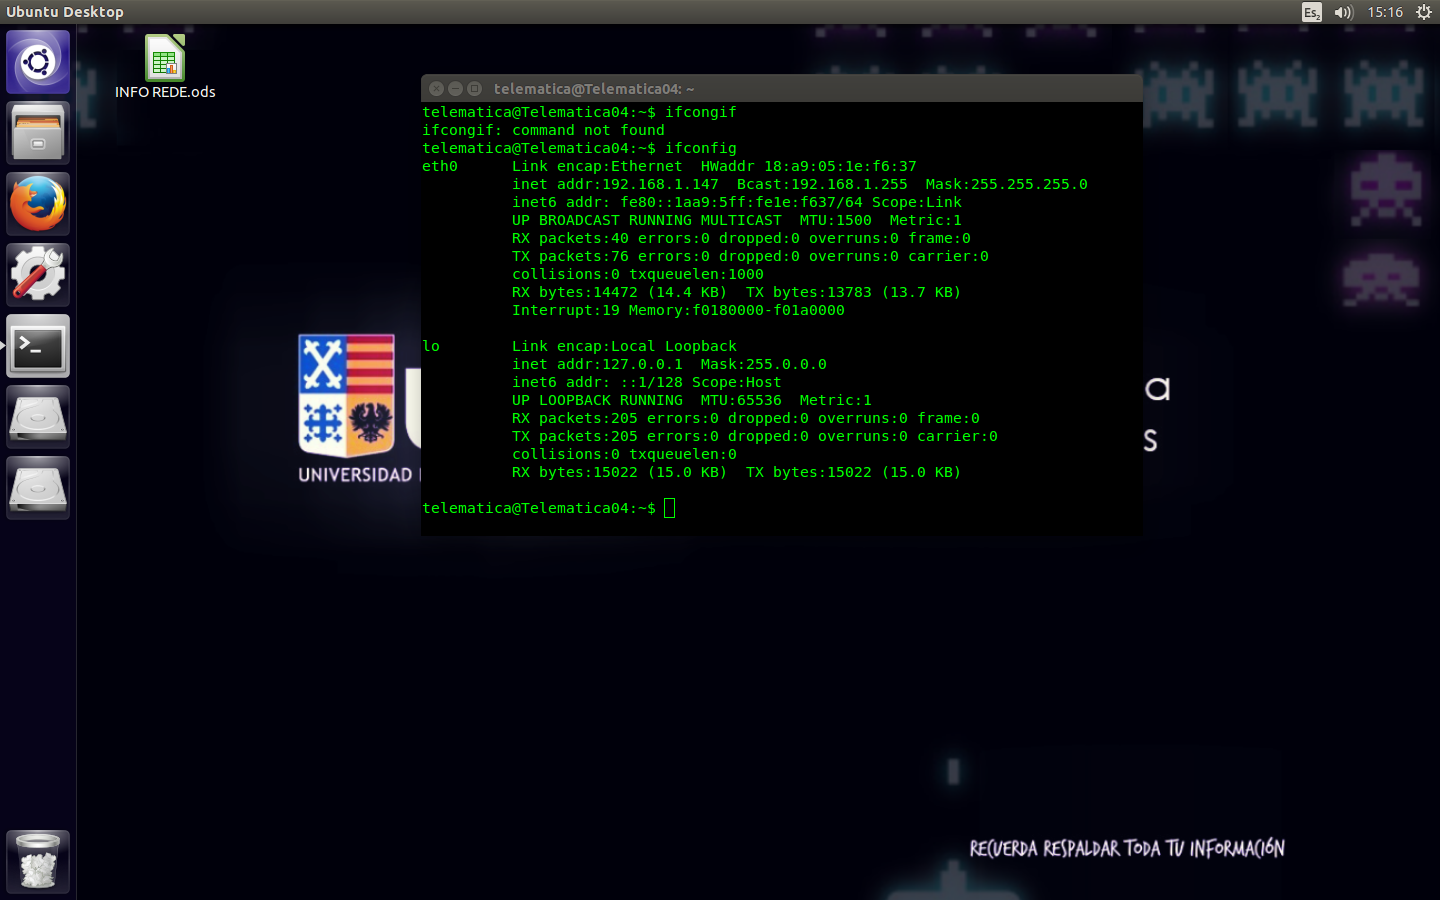
\includegraphics[width=\textwidth]{Terminal.png}
		\end{figure}
		(imagen referencial tomada de otro laboratorio.)\\
		Si observamos la imagen lo que está encerrado en un círculo rojo representa la MAC del equipo y lo encerrado en un
		círculo azul representa la IP del mismo. Al repetir este proceso en cada uno de los computadores de la sala nos    
		dimos cuenta que tanto la MAC como la IP seguían un patrón, en el caso de la MAC los 3 primeros pares de caracteres
		eran iguales en todos los equipos, esto nos dice que las tarjetas de red de todos ellos son del mismo fabricane,      
		el prefijo que se repite es el 40:A8:F0 por lo tanto pudimos llegar a la conclusión de que Hewlett Packard es el      
		fabricante de estas. En el caso de la dirección IP de los computadores solo diferían en los 3 últimos dígitos, ya     
		que al ser una red interna el último número de la dirección debe ser distinto para cada equipo para de esta manera    
		identificar a cada uno.
	\section{Diagrama de red}
		\includegraphics[width=\textwidth]{diagramaf.png}
		Como se observa en el diagrama de red, los computadores están conectados por un cable de red uno por uno 
		a van conectados a el patch, el cual hara que los cables se ubiquen con una mejor distribucion fisica 
		en el espacio.\\
		Gracias a esta descripcion se plantea que la topologia utilizada en el laboratorio de informática
		Este sistema es muy costoso siendo comparado junto con las topologias de anillo o tren, ya que para poder
		conectar cada dispositivo a el switch se necesita un cable nuevo de el mismo tamaño,pero al mismo tiempo
		aporta una caracteristica muy importante la cual es una facil deteccion de problemas y si es que algun
		cable de red se llegara a romper o a tener problemas solo perdera la conexión  ese dispositivo.Aun así 
		si es que el switch llegara a dañarse de alguna forma esto afectaria a el sistema completo ya que solo
		depende de éste.
\chapter{Conclusión}
                Gracias a esta experiencia en el laboratorio hemos logrado comprender como funciona un sistema de redes completo 
                incluyendo sus principales componentes, como los cables de red, el patch panel y el switch, la forma en la cual son 
                conectados estos mismos y las topologías que se podrían haber implementado en la configuración de las conexiones. La 
                topología que se está utilizando en el laboratorio de informática es la que según los integrantes del grupo, es la que
                se adecua a las necesidades existentes, aunque esta requiera de un presupuesto más alto. Además se genera un "orden 
                lógico" entre los dispositivos de redes al poseer en la sala solamente equipos de un mismo modelo.
\end{document}
